\documentclass[11pt]{standalone}
\usepackage{pgf, tikz}
\usetikzlibrary{arrows, automata}
\usetikzlibrary{backgrounds}

\begin{document}
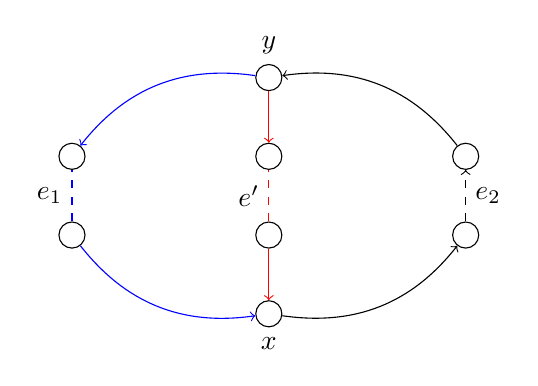
\begin{tikzpicture} [align=center]
\path (0,0) node[circle, draw] (v0) {}
      (0,1) node[circle, draw] (v1) {}
      (2.5,-1) node[circle, draw, label={below:$x$}] (v2) {}
      (2.5,0) node[circle, draw] (v3) {}
      (2.5,1) node[circle, draw] (v4) {}
      (2.5,2) node[circle, draw, label={above:$y$}] (v5) {}
      (5,0) node[circle, draw] (v6) {}
      (5,1) node[circle, draw] (v7) {};

\draw[dashed, blue] (v0) to node[black, left] {$e_1$} (v1);
\draw[dashed, red] (v3) to node[black, left] {$e'$} (v4);
\draw[dashed, ->] (v6) to node[right] {$e_2$} (v7);
\draw[blue, ->] (v0) to [bend right] (v2);
\draw[blue, <-] (v1) to [bend left] (v5);
\draw[red, <-] (v2) to (v3);
\draw[red, <-] (v4) to (v5);
\draw[->] (v2) to [bend right] (v6);
\draw[<-] (v5) to [bend left] (v7);

\end{tikzpicture}
\end{document}